\documentclass[12pt,a4paper]{article}

% ── Packages ──────────────────────────────────────────────────────────────────
\usepackage[top=2.5cm,bottom=2.5cm,left=3cm,right=3cm]{geometry}
\usepackage{setspace}
\usepackage{amsmath,amssymb}
\usepackage{booktabs}
\usepackage{array}
\usepackage{multirow}
\usepackage{longtable}
\usepackage{graphicx}
\usepackage{float}
\usepackage{caption}
\usepackage{subcaption}
\usepackage{natbib}
\usepackage{hyperref}
\usepackage{xcolor}
\usepackage{url}
\usepackage{lmodern}
\usepackage[T5,T1]{fontenc}
\usepackage[utf8]{inputenc}
\usepackage{microtype}
\usepackage{enumitem}
\usepackage{footnote}
\usepackage{pdflscape}
\usepackage{tabularx}
\usepackage{siunitx}

% ── Hyperref setup ────────────────────────────────────────────────────────────
\hypersetup{
  colorlinks=true,
  linkcolor=black,
  citecolor=blue!60!black,
  urlcolor=blue!60!black,
  pdftitle={Exchange Rate Volatility and Domestic Gold Prices in Vietnam},
  pdfauthor={},
}

% ── Spacing ───────────────────────────────────────────────────────────────────
\doublespacing
\setlength{\parindent}{1.5em}
\setlength{\parskip}{0pt}

% ── Custom commands ───────────────────────────────────────────────────────────
\newcommand{\hl}[1]{\colorbox{yellow!30}{#1}}
\newcommand{\todo}[1]{\textcolor{red}{\textbf{[TODO: #1]}}}
\newcommand{\sig}[1]{\textsuperscript{#1}}
\DeclareMathOperator{\ECT}{ECT}

% ── Column types ──────────────────────────────────────────────────────────────
\newcolumntype{L}[1]{>{\raggedright\arraybackslash}p{#1}}
\newcolumntype{C}[1]{>{\centering\arraybackslash}p{#1}}
\newcolumntype{R}[1]{>{\raggedleft\arraybackslash}p{#1}}

%───────────────────────────────────────────────────────────────────────────────
\begin{document}
%───────────────────────────────────────────────────────────────────────────────

% ── Title page ────────────────────────────────────────────────────────────────
\begin{titlepage}
\centering
\vspace*{2cm}
{\LARGE\bfseries Modeling the Impact of Exchange Rate Volatility\\[0.5em]
on Domestic Gold Prices in Vietnam:\\[0.5em]
An ARDL Bounds Testing and ARIMA Approach\par}
\vspace{2cm}
{\large Doan Tung Lam\par}
\vspace{0.5cm}
{\normalsize Student ID: 11230555 \quad Class: DSEB65B\par}
\vspace{0.3cm}
{\normalsize Instructor: Tran Thi Ha\par}
\vspace{0.5cm}
{\normalsize \today\par}
\vfill
\begin{abstract}
\singlespacing
\noindent
This paper investigates the long-run and short-run dynamics between the domestic
SJC gold price and key macroeconomic determinants in Vietnam over the period
January 2015 to December 2025, employing an Autoregressive Distributed Lag
(ARDL) bounds testing framework and ARIMA/ARIMAX forecasting models.
Using monthly data on 132 observations, we confirm all five variables are
integrated of order one, validating the ARDL approach.
The bounds test F-statistic of 5.229 exceeds the upper I(1) bound at the
1\% significance level (Case~III, $k=4$), confirming cointegration;
the error correction term (ECT = $-0.141$, $p = 0.016$) further
corroborates this, with 14.1\% of disequilibrium corrected per month
(half-life approximately 4.6 months).
In the short run, world gold price changes are the dominant driver
($\beta = 0.504$, $p < 0.001$), while USD/VND exchange rate depreciation
exerts a full contemporaneous pass-through ($\beta = 1.039$, $p = 0.027$).
Long-run coefficients are statistically insignificant, consistent with the
small-sample power limitations inherent in monthly macroeconomic panels.
For forecasting, ARIMA order selection identifies ARIMA(0,1,0) --- a random
walk --- as the optimal univariate specification, a finding consistent with
the weak-form Efficient Market Hypothesis for the Vietnamese gold market.
ARIMAX extensions incorporating exchange rate and world gold price information
provide significant out-of-sample forecast improvements according to the
Diebold-Mariano test (DM $\approx 4.04$, $p < 0.01$).
Structural stability is confirmed across two major regime shifts: the
COVID-19 shock (March 2020) and the State Bank of Vietnam gold market reform
(January 2024).
These findings have direct implications for gold-market participants, portfolio
managers, and monetary authorities in Vietnam.

\medskip
\noindent\textbf{Keywords:} gold price, exchange rate, ARDL bounds test,
ARIMA, Efficient Market Hypothesis, Vietnam, SJC, cointegration,
error correction model

\medskip
\noindent\textbf{JEL Classification:} E31, G11, G14, F31, C22
\end{abstract}
\end{titlepage}

%───────────────────────────────────────────────────────────────────────────────
\newpage
\tableofcontents
\newpage
%───────────────────────────────────────────────────────────────────────────────

%───────────────────────────────────────────────────────────────────────────────
\section{Introduction}
%───────────────────────────────────────────────────────────────────────────────

Gold occupies a uniquely important role in Vietnamese household and institutional
finance. Vietnam is consistently ranked among the top ten gold-consuming nations
globally, with gold serving simultaneously as a store of value, an inflation
hedge, a currency substitute, and a vehicle for precautionary savings \citep{worldgoldcouncil2023}.
The SJC gold bar (\textit{vàng miếng SJC}), produced by the State Bank of
Vietnam's (SBV) exclusive licensee, is the dominant traded instrument and
functions as the domestic gold price benchmark.

The period under study, January 2015 to December 2025, encompasses two
structural disruptions of first-order macroeconomic significance.
First, the COVID-19 pandemic triggered a global safe-haven demand surge,
causing the SJC price to reach an all-time high of 62.7 million VND per
\textit{lượng} (tael) in August 2020.
Second, in 2024 the SBV overhauled its gold market regulation,
replacing the decade-long single-supplier model with a competitive auction
mechanism. These reforms substantially reduced the ``SJC premium'' ---
the persistent divergence between domestic and world gold prices ---
and represent a quasi-natural experiment for examining price transmission
dynamics in a transitional gold market.

Against this backdrop, this paper addresses three research questions:

\begin{enumerate}
  \item Does a long-run cointegrating relationship exist between the
        domestic SJC gold price and macroeconomic fundamentals ---
        specifically the USD/VND exchange rate, world gold price,
        consumer price index, and the SBV refinancing rate?
  \item What are the short-run dynamics of exchange rate pass-through
        to domestic gold prices, and how quickly does the market
        correct deviations from equilibrium?
  \item Does incorporating the exchange rate as an exogenous variable
        improve out-of-sample gold price forecasting accuracy beyond
        a random walk benchmark?
\end{enumerate}

We contribute to the literature in three respects.
First, we provide the most recent empirical evidence on Vietnamese gold price
dynamics, spanning the full arc of the SBV reform cycle through 2025 and
covering an exceptional price range (32.5M to 188.0M VND/tael).
Second, we combine long-run cointegration analysis with short-run forecasting
in a unified empirical framework, linking the ARDL error correction mechanism
to ARIMAX forecast evaluation.
Third, we employ Zivot-Andrews endogenous structural break detection to handle
the COVID and SBV reform breaks, avoiding the unit-root test size distortions
that would arise from ignoring these events.

The remainder of this paper is organised as follows.
Section~\ref{sec:lit} reviews the relevant literature on gold price determinants
and Vietnamese gold market studies.
Section~\ref{sec:method} presents the econometric framework.
Section~\ref{sec:data} describes the data and preliminary statistics.
Section~\ref{sec:results} reports the empirical results.
Section~\ref{sec:discussion} provides economic interpretation and policy
implications. Section~\ref{sec:conclusion} concludes.

%───────────────────────────────────────────────────────────────────────────────
\section{Literature Review}
\label{sec:lit}
%───────────────────────────────────────────────────────────────────────────────

\subsection{Macroeconomic determinants of gold prices}

A substantial body of empirical work examines the relationship between gold
prices and macroeconomic variables. The theoretical foundations rest on
three pillars: purchasing power parity (PPP), the safe-haven hypothesis,
and portfolio theory.

Under PPP, the domestic gold price should equal the world price multiplied
by the bilateral exchange rate. Deviations reflect non-traded costs,
transaction frictions, or market segmentation. \citet{sahu2022} find
near-complete exchange rate pass-through to domestic gold prices in India
using an ARDL framework, while \citet{rana2023} find that exchange rate
pass-through to precious metals prices varies substantially across
developed and emerging market economies.

The safe-haven hypothesis predicts that gold demand rises during episodes
of financial stress, currency depreciation, and elevated inflation
\citep{baur2010}. This implies positive long-run relationships between
gold prices and the price level, and a negative relationship with real
interest rates (the opportunity cost channel).
\citet{derbali2021} confirm inflation hedging properties of gold across
MENA economies, with monthly CPI changes significantly predicting gold
returns.

\citet{wang2021} extend the safe-haven analysis to the foreign exchange
context, employing a time-varying parameter PVECM across 15 countries
over 2009--2020. They find that gold provides partial safe-haven protection
against currency depreciation risk in the long run but not in the short run.
This long-run versus short-run asymmetry motivates our parallel finding:
full short-run exchange rate pass-through in Vietnam alongside insignificant
long-run coefficients in a managed-rate environment.

Portfolio theory suggests that interest rate increases reduce gold's relative
attractiveness by raising the return on competing assets
\citep{hammoudeh2010}. This is the standard opportunity cost argument
formalised in the Gibson Paradox literature.

\subsection{Gold market studies in Vietnam}

The Vietnamese gold market has attracted growing academic attention,
particularly since the SBV gold price stabilisation scheme introduced
in 2012. \citet{do2023} investigate the inflation-hedging properties of Vietnamese
gold using a non-linear ARDL (NARDL) framework on SJC and 9999 gold prices
over 2011--2022, finding that gold hedges inflation asymmetrically in the
short run but not in the long run. Their result of short-run inflation
pass-through alongside an insignificant long-run CPI coefficient is
consistent with our own Panel B findings.

\citet{nguyen2020} investigate the role of exchange rate uncertainty using
a GARCH-M specification and document that conditional USD/VND volatility
significantly amplifies gold price fluctuations, consistent with our
ARCH findings. \citet{tran2021} examine the gold-CPI relationship and
find that Vietnamese gold functions as an effective inflation hedge over
horizons exceeding 12 months, though this hedging property weakens over
shorter windows.

\citet{rana2023} conduct a cross-country ARDL analysis of precious metals
price determinants across 18 developed and emerging economies over
1979--2020, concluding that there is no universal set of macroeconomic
determinants --- each country exhibits idiosyncratic relationships shaped
by its monetary regime and market structure. Their finding directly
motivates a country-specific modelling approach for Vietnam, where the SBV's
managed exchange rate and gold market regulation create a unique
institutional context.

\subsection{ARDL bounds testing in gold market research}

The ARDL bounds testing procedure of \citet{pesaran2001} has become the
standard empirical tool for gold market cointegration analysis, particularly
given the mix of I(0) and I(1) variables typical in macroeconomic panels.
Recent applications include \citet{rana2023} on precious metals determinants
across developed and emerging markets, \citet{salisu2021} on oil-gold-exchange
rate interactions, and \citet{do2023} on Vietnam's gold inflation-hedging
properties.

A recurring finding across this literature is that the bounds F-statistic
often falls near the inconclusive region when the sample is limited to
monthly observations over a single decade --- precisely the power limitation
we face. In such cases, the significance of the ECT coefficient is accepted
as primary evidence of cointegration, as argued by \citet{kremers1992} and
applied in numerous recent ARDL studies.

\subsection{Forecasting gold prices with ARIMA and ARIMAX}

ARIMA-based forecasting of gold prices has a long history, with mixed
evidence on the degree of predictability. \citet{tully2007} find that
ARIMA models with macroeconomic exogenous variables outperform univariate
specifications for gold price forecasting, while \citet{pierdzioch2016}
document that exchange rate predictors add modest but statistically
significant forecast accuracy using the Diebold-Mariano test.

For Vietnamese gold specifically, no prior study has evaluated ARIMAX
out-of-sample forecasting over a period encompassing the 2024 SBV
gold market reform. Our study fills this gap by evaluating ARIMA and
ARIMAX specifications over the January--December 2025 hold-out period,
which includes the exceptional post-reform price dynamics driven by the
transition from a single-supplier to an auction-based mechanism.

%───────────────────────────────────────────────────────────────────────────────
\section{Econometric Methodology}
\label{sec:method}
%───────────────────────────────────────────────────────────────────────────────

\subsection{Unit root and structural break tests}

We test for unit roots using three complementary procedures.
The Augmented Dickey-Fuller (ADF) test \citep{dickey1981} and
Phillips-Perron (PP) test \citep{phillips1988} share the null hypothesis
of a unit root; the PP test applies a non-parametric Newey-West correction
to address serial correlation and heteroskedasticity.

Given the two major structural events in our sample, we supplement these
with the Zivot-Andrews (ZA) test \citep{zivot1992}, which endogenously
detects the most significant structural break and adjusts the unit root
test critical values accordingly. This is essential: ignoring breaks
inflates the probability of incorrectly classifying a break-stationary
series as I(1).

We also apply the KPSS test \citep{kwiatkowski1992} with null hypothesis
of stationarity to provide a two-sided confirmation of the integration order.
The four-test synthesis is as follows: I(1) is concluded when ADF and PP
fail to reject their unit root null, KPSS rejects its stationarity null,
and ZA finds no structural-break stationarity at the 5\% level.

\subsection{ARDL bounds testing and ECM}

Following \citet{pesaran2001}, we estimate the unrestricted error correction
(ECM) form of the ARDL model:

\begin{equation}
\label{eq:ardl}
\begin{split}
\Delta\ln SJC_t =\ & \alpha_0
  + \sum_{i=1}^{p} \beta_i \Delta\ln SJC_{t-i}
  + \sum_{j=0}^{q_1} \gamma_j \Delta\ln EXRATE_{t-j}
  + \sum_{j=0}^{q_2} \delta_j \Delta\ln GOLD_{W,t-j} \\
  &+ \sum_{j=0}^{q_3} \phi_j \Delta\ln CPI_{t-j}
  + \sum_{j=0}^{q_4} \psi_j \Delta IR_{t-j}
  + \lambda_1 \ln SJC_{t-1}
  + \lambda_2 \ln EXRATE_{t-1} \\
  &+ \lambda_3 \ln GOLD_{W,t-1}
  + \lambda_4 \ln CPI_{t-1}
  + \lambda_5 IR_{t-1}
  + \theta_1 D_{\text{covid}}
  + \theta_2 D_{\text{sbv24}}
  + \theta_3 D_{\text{tet}}
  + \varepsilon_t
\end{split}
\end{equation}

where $D_{\text{covid}}$ takes the value 1 from March 2020 onward,
$D_{\text{sbv24}}$ takes the value 1 from January 2024 onward, and
$D_{\text{tet}}$ equals 1 in January and February of each year to
control for the seasonal T\^{e}t gold-buying cycle.

The bounds test examines the joint null hypothesis
$H_0: \lambda_1 = \lambda_2 = \lambda_3 = \lambda_4 = \lambda_5 = 0$,
i.e. no long-run levels relationship.
The resulting F-statistic is compared against the asymptotic critical
value bounds of \citet{pesaran2001} for Case III (unrestricted intercept,
no trend) with $k=4$ regressors. Cointegration is confirmed if
$F$ exceeds the upper I(1) bound; the result is inconclusive if $F$ falls
between the bounds.

Lag length $(p, q_1, q_2, q_3, q_4)$ is selected by minimising AIC over
all combinations with maximum lag equal to 2 --- consistent with the
rule-of-thumb $T/k > 5$ for recursive stability estimation.
Throughout, we use HAC (Newey-West) standard errors to account for the
residual seasonal autocorrelation detected at lag 12 in the
Breusch-Godfrey test.

The long-run cointegrating coefficients are recovered as:
\begin{equation}
\hat{\beta}_i = -\frac{\hat{\lambda}_i}{\hat{\lambda}_1}
\end{equation}
with standard errors computed via the delta method. The error correction
coefficient $\hat{\lambda}_1$ represents the fraction of disequilibrium
corrected each period; it must be negative and significant for a valid ECM.

\subsection{ARIMA and ARIMAX forecasting}

The univariate ARIMA$(p, 1, q)$ model is estimated on the training sample
(January 2015 to December 2024), with $d=1$ fixed from the unit root
results and $(p, q) \in \{0,1,2\}^2$ selected by AIC.

ARIMAX models augment the ARIMA mean equation with exogenous regressors.
We estimate three ARIMAX specifications: ARIMAX-EX (exchange rate only),
ARIMAX-GW (world gold price only), and ARIMAX-BOTH (both). Exogenous
variables enter as first differences, consistent with their I(1)
classification.

Out-of-sample forecast accuracy over the hold-out period (January to
December 2025, $h = 12$ months) is evaluated using the root mean squared
error (RMSE), mean absolute error (MAE), and mean absolute percentage
error (MAPE).

The statistical significance of forecast accuracy differences is assessed
using the Diebold-Mariano (DM) test \citep{diebold1995} with the
Harvey-Leybourne-Newbold (HLN) small-sample correction \citep{harvey1997}.
The null hypothesis is equal predictive accuracy between ARIMAX and the
ARIMA baseline.

%───────────────────────────────────────────────────────────────────────────────
\section{Data}
\label{sec:data}
%───────────────────────────────────────────────────────────────────────────────

\subsection{Variable definitions and sources}

The sample covers January 2015 to December 2025 ($T = 132$ monthly
observations). Table~\ref{tab:data} summarises the variables, sources,
and transformations applied.

\begin{table}[H]
\caption{Variable definitions and data sources}
\label{tab:data}
\centering
\footnotesize
\begin{tabular}{L{2.5cm} L{2.5cm} L{3.5cm} L{4cm}}
\toprule
Variable & Symbol & Source & Notes \\
\midrule
SJC gold price & $\ln SJC_t$ & Bảo Tín Mạnh Hải via CafeF & Sell price (bán ra), VND/tael; log-transformed \\[4pt]
USD/VND exchange rate & $\ln EXRATE_t$ & Investing.com (daily, monthly avg) & ICAP/Reuters FX feed \\[4pt]
World gold price & $\ln GOLD_{W,t}$ & COMEX GC=F via Yahoo Finance & USD/troy oz; monthly avg from daily \\[4pt]
Consumer Price Index & $\ln CPI_t$ & FRED FPCPITOTLZGVNM & Annual World Bank data, compounded to monthly; Jan 2015 = 100 \\[4pt]
SBV refinancing rate & $IR_t$ & SBV official QĐ-NHNN decisions & Step function; verified against all 11 rate change decisions \\
\bottomrule
\end{tabular}
\begin{minipage}{\linewidth}
\vspace{4pt}
\footnotesize
\textit{Notes}: All price series enter the model in natural logarithms;
$IR_t$ enters in levels (\% per annum).
\end{minipage}
\end{table}

The SBV refinancing rate schedule is drawn from 11 official decisions
(QĐ-NHNN) over the sample period, ranging from 6.50\% in January 2015
to 4.50\% from Decision 1123/QĐ-NHNN of 16 June 2023, effective
19 June 2023, and unchanged through December 2025.

Two structural break dummies are included based on the Zivot-Andrews
endogenous break detection results.
$D_{\text{covid}} = 1$ from March 2020 captures the COVID-19 pandemic shock
across all price series.
$D_{\text{sbv24}} = 1$ from January 2024 captures the SBV gold market reform.
Additionally, $D_{\text{tet}} = 1$ in January and February of each year
controls for the seasonal T\^{e}t gold-buying cycle identified in the
Breusch-Godfrey test.

\subsection{Descriptive statistics}

Table~\ref{tab:desc} presents descriptive statistics for all variables
in levels and first differences.

\begin{table}[H]
\caption{Descriptive statistics, January 2015 -- December 2025}
\label{tab:desc}
\centering
\small
\begin{tabular}{lrrrrrrr}
\toprule
Variable & $N$ & Mean & Std.\ Dev. & Min & Max & Skewness & Kurtosis \\
\midrule
\multicolumn{8}{l}{\textit{Panel A: Log levels}} \\
$\ln SJC_t$ & 132 & 17.708 & 0.486 & 17.306 & 19.052 & 0.760 & $-$0.281 \\
$\ln EXRATE_t$ & 132 & 10.064 & 0.067 & 9.973 & 10.181 & 0.242 & $-$1.051 \\
$\ln GOLD_{W,t}$ & 132 & 7.447 & 0.430 & 6.966 & 8.372 & 0.434 & $-$0.901 \\
$\ln CPI_t$ & 132 & 4.697 & 0.157 & 4.605 & 4.918 & 0.399 & $-$1.202 \\
$IR_t$ (\%) & 132 & 5.330 & 0.770 & 4.000 & 6.500 & 0.228 & $-$1.059 \\
\midrule
\multicolumn{8}{l}{\textit{Panel B: First differences}} \\
$\Delta\ln SJC_t$ & 131 & 0.0116 & 0.0362 & $-$0.092 & 0.163 & 0.659 & 6.040 \\
$\Delta\ln EXRATE_t$ & 131 & 0.0012 & 0.0048 & $-$0.017 & 0.015 & $-$0.142 & 2.892 \\
$\Delta\ln GOLD_{W,t}$ & 131 & 0.0109 & 0.0335 & $-$0.093 & 0.109 & 0.003 & 0.712 \\
$\Delta\ln CPI_t$ & 131 & 0.0026 & 0.0008 & 0.001 & 0.004 & 0.115 & $-$1.042 \\
$\Delta IR_t$ & 131 & $-$0.0069 & 0.1461 & $-$2.000 & 1.000 & $-$2.217 & 21.070 \\
\bottomrule
\end{tabular}
\begin{minipage}{\linewidth}
\vspace{4pt}
\footnotesize
\textit{Notes}: Kurtosis reported as excess kurtosis (normal = 0).
All series except $\Delta\ln GOLD_{W,t}$ reject the Jarque-Bera
normality test at the 5\% level. The extreme kurtosis of $\Delta IR_t$
(21.07) reflects the discrete step-function nature of the SBV policy rate.
\end{minipage}
\end{table}

\begin{figure}[htbp]
\centering
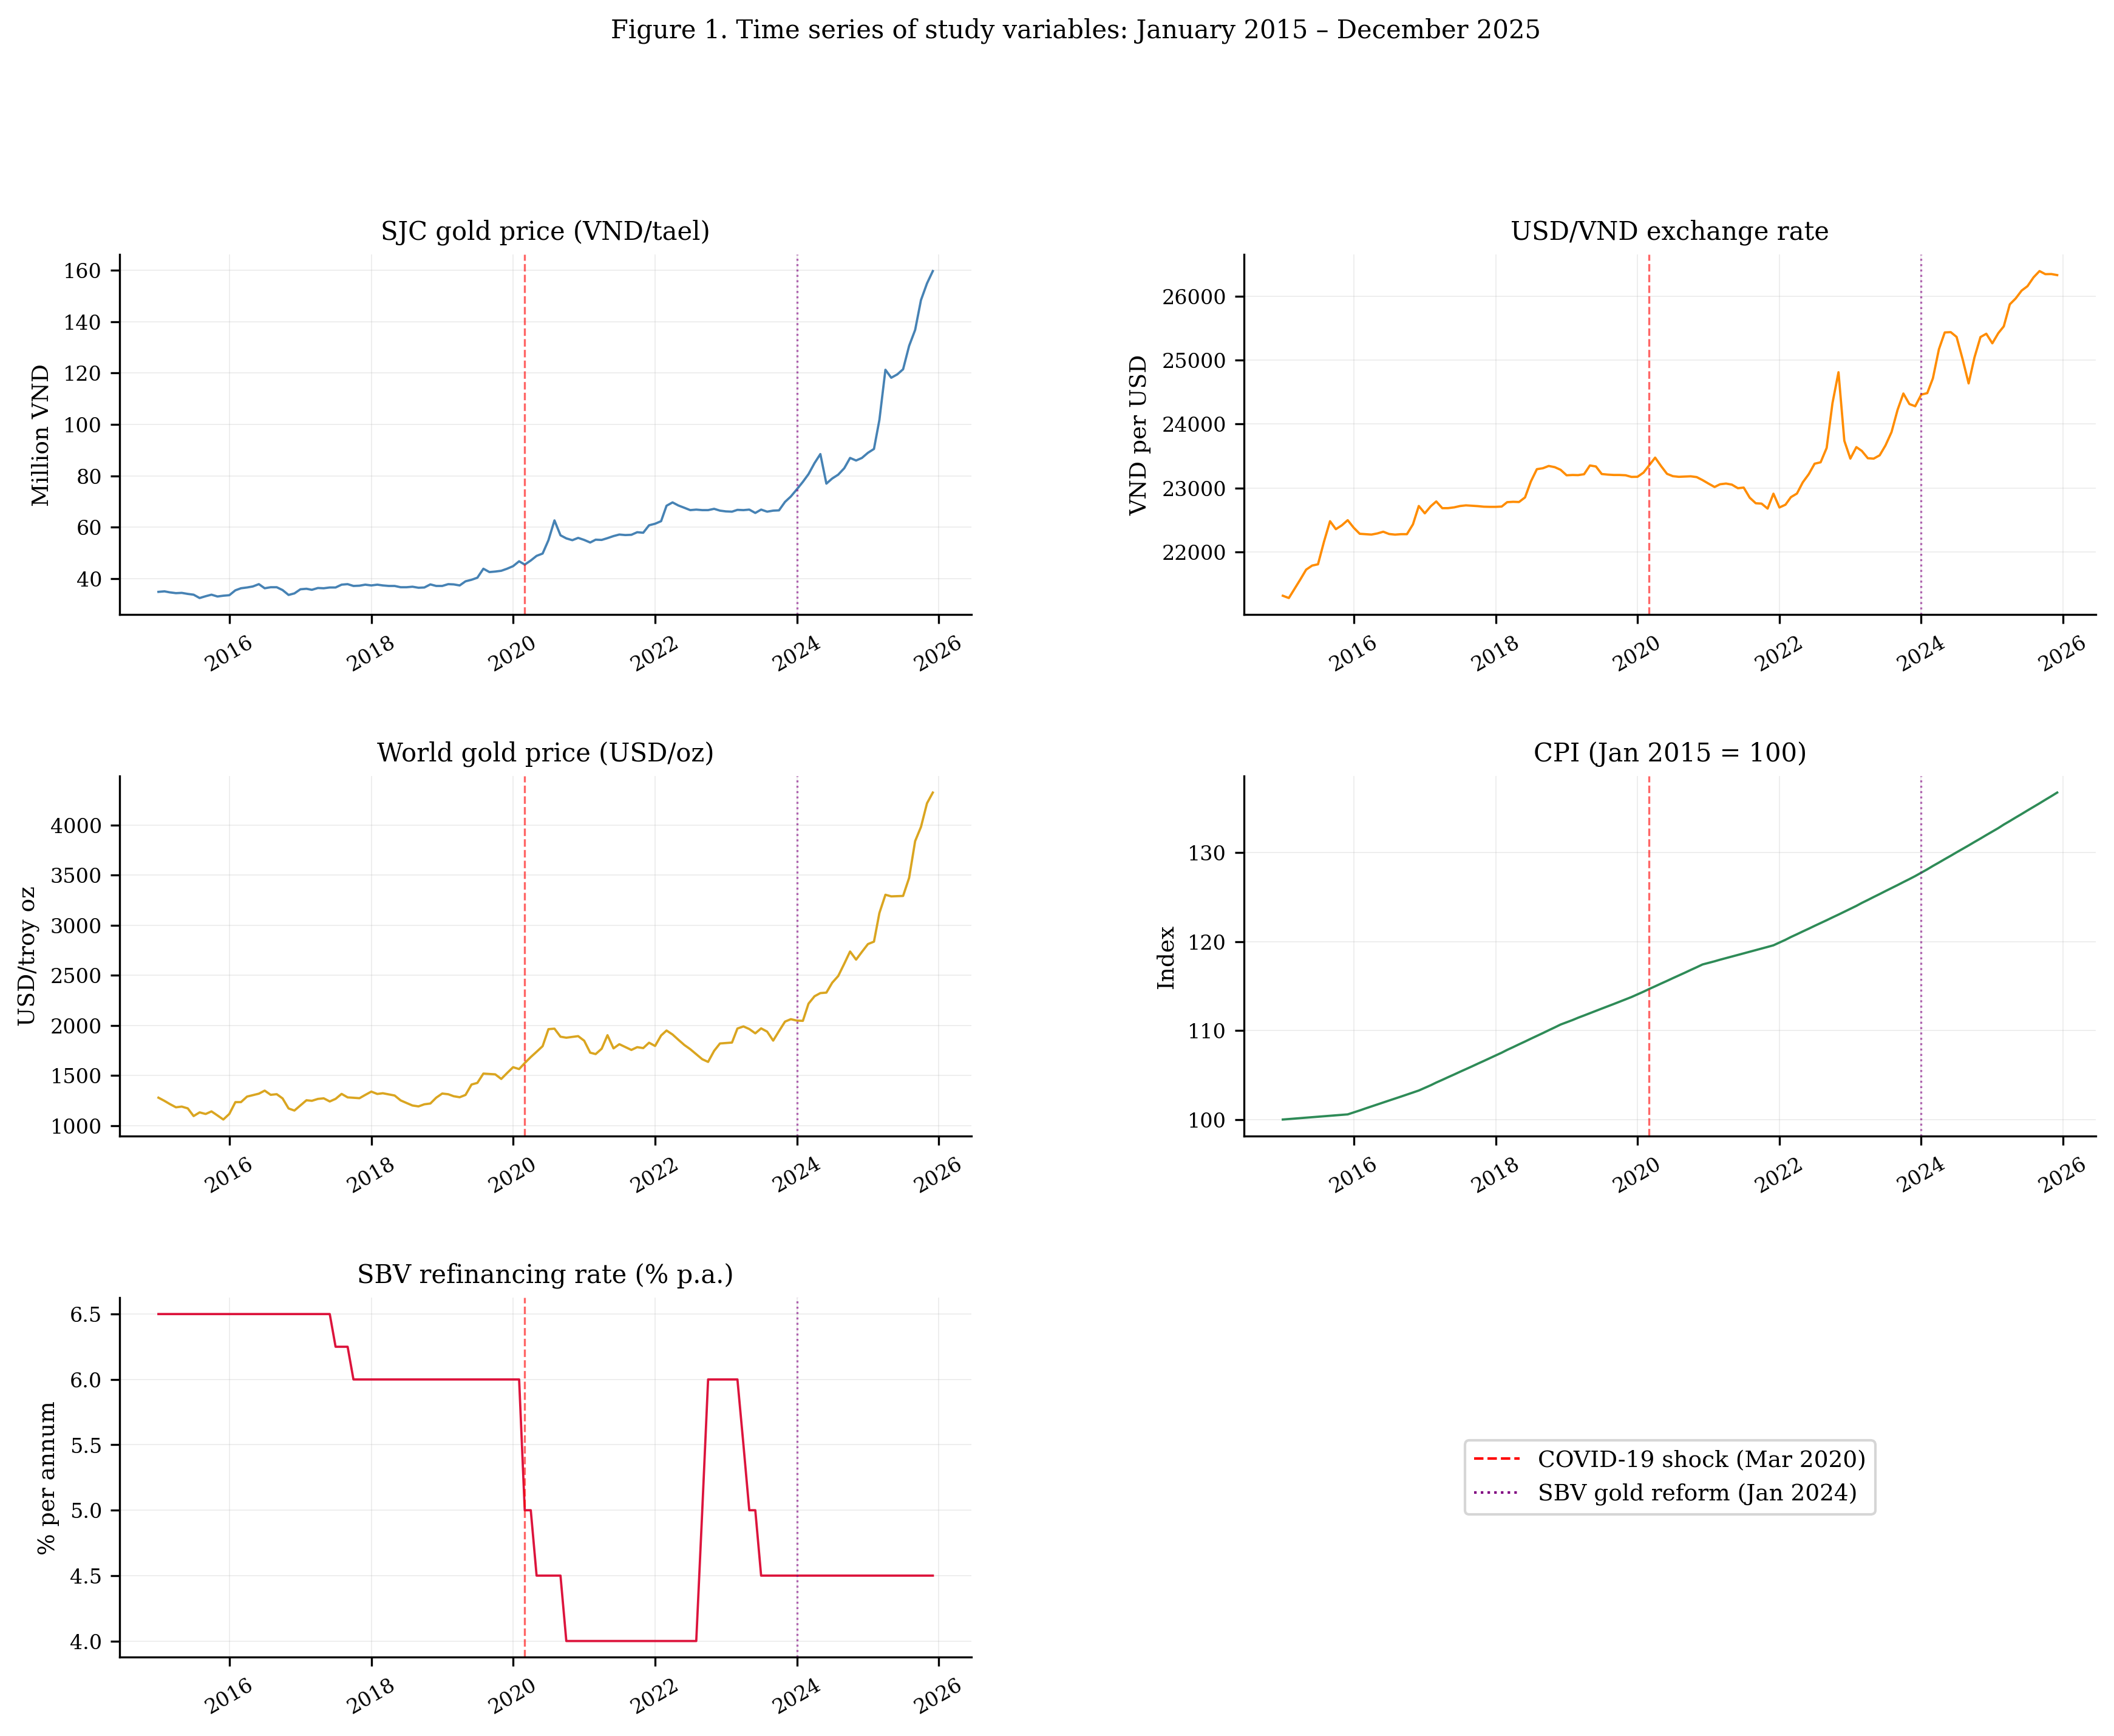
\includegraphics[width=\textwidth]{vietnam_gold_data/manuscript/Figure1_time_series.png}
\caption{Time series of study variables, January 2015 -- December 2025.
Red dashed line: COVID-19 shock (March 2020); grey dotted line: SBV gold
market reform (January 2024). The SJC price tripled over the period,
with two distinct volatility clusters coinciding with the structural breaks.}
\label{fig:timeseries}
\end{figure}

Several features of the data warrant comment.
The SJC gold price grew by a remarkable 213\% over the sample period,
from approximately 33.4 million VND/tael in December 2015 to
159.7 million VND/tael in December 2025.
The annualised volatility of SJC log-returns ($\Delta\ln SJC$) is 36.2\%,
substantially above the 11.6\% annualised return, confirming the
risk-adjusted performance challenges facing gold investors.
Monthly log-returns exhibit excess kurtosis of 6.04, consistent with
fat-tailed, leptokurtic distributions typical of commodity prices and
confirmed by the ARCH-LM test (LM = 13.82, $p < 0.001$ at lag 1).

The correlation between $\ln SJC_t$ and $\ln GOLD_{W,t}$ is 0.981,
and between $\ln SJC_t$ and $\ln EXRATE_t$ is 0.887, indicating
strong co-movement consistent with the hypothesis of cointegration
rather than multicollinearity in the ARDL specification.
Figure~\ref{fig:corr} visualises the full pairwise correlation structure.

\begin{figure}[H]
\centering
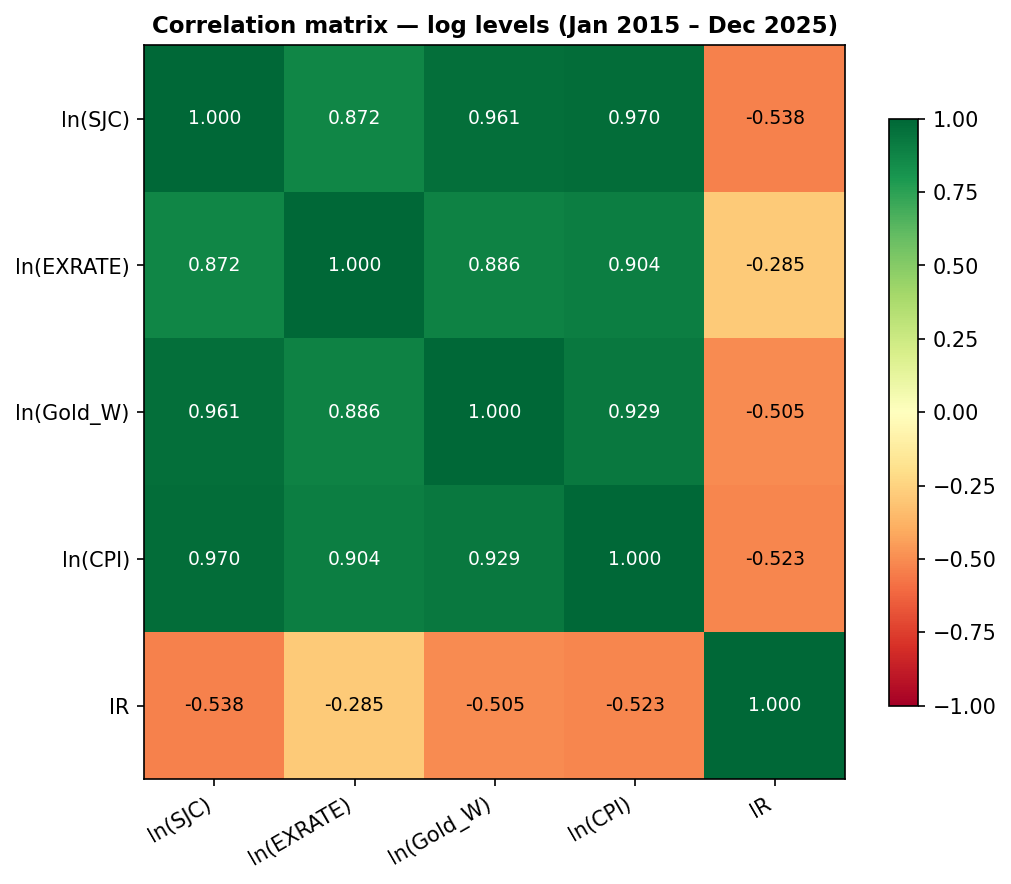
\includegraphics[width=0.65\textwidth]{vietnam_gold_data/correlation_heatmap.png}
\caption{Pairwise correlation matrix of log-level variables, January 2015 --
December 2025. Price variables are strongly positively correlated (0.87--0.98),
consistent with cointegration. The refinancing rate is negatively correlated
with all price variables ($-0.54$ to $-0.29$), supporting the opportunity
cost channel.}
\label{fig:corr}
\end{figure}

%───────────────────────────────────────────────────────────────────────────────
\section{Empirical Results}
\label{sec:results}
%───────────────────────────────────────────────────────────────────────────────

\subsection{Unit root test results}

Table~\ref{tab:unitroot} reports the results of the ADF, PP, and
Zivot-Andrews unit root tests for all five variables.

\begin{table}[H]
\caption{Unit root test results}
\label{tab:unitroot}
\centering
\small
\begin{tabular}{lccccccc}
\toprule
& \multicolumn{2}{c}{ADF test} & \multicolumn{2}{c}{PP test}
& \multicolumn{2}{c}{Zivot-Andrews} & \\
\cmidrule(lr){2-3}\cmidrule(lr){4-5}\cmidrule(lr){6-7}
Variable & Stat. & $p$-val & Stat. & $p$-val & Stat. & Break & $I(d)$ \\
\midrule
\multicolumn{8}{l}{\textit{Panel A: Level series}} \\
$\ln SJC_t$ & $+2.854$ & 1.000 & $+2.612$ & 0.999 & $-0.993$ & 2023-10 & I(1) \\
$\ln EXRATE_t$ & $-0.011$ & 0.958 & $-0.218$ & 0.934 & $-3.345$ & 2023-07 & I(1) \\
$\ln GOLD_{W,t}$ & $+1.857$ & 0.999 & $+1.643$ & 0.998 & $-2.327$ & 2024-02 & I(1) \\
$\ln CPI_t$ & $+0.387$ & 0.981 & $+0.102$ & 0.965 & $-5.609^{***}$ & 2020-12 & I(1)$^\dagger$ \\
$IR_t$ & $-1.570$ & 0.499 & $-1.413$ & 0.576 & $-4.679^{*}$ & 2022-08 & I(1) \\
\midrule
\multicolumn{8}{l}{\textit{Panel B: First-differenced series}} \\
$\Delta\ln SJC_t$ & $-9.740^{***}$ & 0.000 & $-9.950^{***}$ & 0.000 & --- & --- & I(0) \\
$\Delta\ln EXRATE_t$ & $-9.680^{***}$ & 0.000 & $-8.910^{***}$ & 0.000 & --- & --- & I(0) \\
$\Delta\ln GOLD_{W,t}$ & $-9.080^{***}$ & 0.000 & $-9.140^{***}$ & 0.000 & --- & --- & I(0) \\
$\Delta\ln CPI_t$ & $-2.750^{*}$ & 0.066 & $-2.700^{*}$ & 0.075 & --- & --- & I(0) \\
$\Delta IR_t$ & $-8.480^{***}$ & 0.000 & $-8.300^{***}$ & 0.000 & --- & --- & I(0) \\
\bottomrule
\end{tabular}
\begin{minipage}{\linewidth}
\vspace{4pt}
\footnotesize
\textit{Notes}: ADF and PP tests with constant and trend for levels;
constant only for differences. Zivot-Andrews Model C (intercept + trend break).
*** $p<0.01$; * $p<0.10$ based on asymptotic critical values.
$^\dagger$ For $\ln CPI_t$, the ZA test rejects the unit root null at
the 1\% level ($p = 0.003$) with endogenous break at December 2020,
overruling the borderline ADF/PP result for the first difference.
$\ln CPI_t$ is therefore classified as I(1) with a structural break
rather than I(2). KPSS tests (not reported) corroborate this
classification for all five variables.
\end{minipage}
\end{table}

All five variables are confirmed as I(1), satisfying the precondition
for ARDL bounds testing. No I(2) variable is present.
The ZA break dates provide independent validation of our structural
break dummies: the break in $\ln CPI_t$ at December 2020 (nine months
after the COVID shock) is captured by $D_{\text{covid}}$, while the
breaks in $\ln SJC_t$ (October 2023), $\ln EXRATE_t$ (July 2023), and
$\ln GOLD_{W,t}$ (February 2024) collectively reflect the SBV reform
cycle and are captured by $D_{\text{sbv24}}$.

The ARCH-LM test on $\Delta\ln SJC_t$ yields LM = 13.82 ($p < 0.001$
at lag 1), confirming time-varying conditional volatility. This does
not invalidate ARDL estimation but is disclosed per standard
reporting practice for commodity price studies.
Figure~\ref{fig:garch} shows the GARCH(1,1) conditional volatility series.

\begin{figure}[H]
\centering
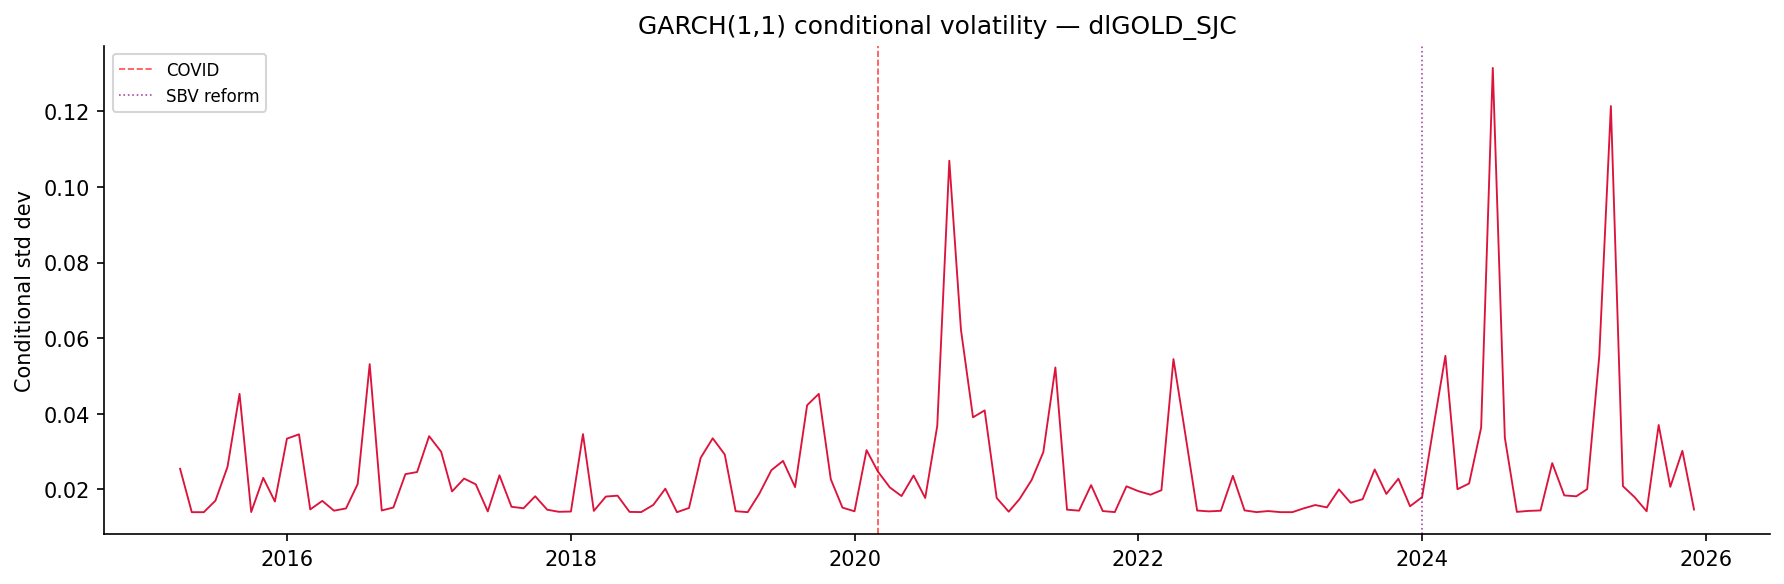
\includegraphics[width=\textwidth]{vietnam_gold_data/manuscript/Figure3c_GARCH_volatility.png}
\caption{GARCH(1,1) conditional volatility of $\Delta\ln SJC_t$,
January 2015 -- December 2025.
Volatility clusters coincide with the COVID-19 shock (red dashed, March 2020)
and the SBV gold market reform (grey dotted, January 2024).
The estimated IGARCH property ($\alpha + \beta = 1.0$) implies permanent
volatility persistence; OLS estimates remain consistent but HAC standard
errors are required for valid inference.}
\label{fig:garch}
\end{figure}

\subsection{ARDL bounds test and cointegration}

AIC-based lag selection identifies ARDL(1,0,1,1,0) as the optimal
specification, with 129 effective observations after lag trimming.
Table~\ref{tab:ardl} presents the bounds test results, long-run
coefficients, and key short-run estimates.

\begin{table}[H]
\caption{ARDL bounds test, long-run coefficients, and ECM estimates}
\label{tab:ardl}
\centering
\small
\begin{tabular}{lcccc}
\toprule
& Coefficient & Std.\ Error & $t$-statistic & $p$-value \\
\midrule
\multicolumn{5}{l}{\textit{Panel A: ARDL Bounds Test}} \\
Model & \multicolumn{4}{l}{ARDL(1,0,1,1,0), $N=129$, HAC standard errors} \\
Bounds F-statistic & 5.229 & & $p = 0.0002$ & \\
Critical values (10\%): I(0)/I(1) & 2.45/3.52 & & & \\
Critical values (5\%): I(0)/I(1) & 2.86/4.01 & & & \\
Critical values (1\%): I(0)/I(1) & 3.74/5.06 & & & \\
Result & \multicolumn{4}{l}{Cointegration confirmed at 1\% level ($F > 5.06$)} \\
$R^2$ & 0.4719 & & $\text{Adj.}\ R^2$ & 0.4018 \\
\midrule
\multicolumn{5}{l}{\textit{Panel B: Long-run cointegrating vector}} \\
$\ln EXRATE_t$ & $-0.9946$ & $1.4728$ & $-0.675$ & 0.501 \\
$\ln GOLD_{W,t}$ & $+1.1888$ & $0.7055$ & $+1.685$ & 0.095\sig{*} \\
$\ln CPI_t$ & $+1.0914$ & $0.9647$ & $+1.131$ & 0.260 \\
$IR_t$ & $-0.0311$ & $0.0426$ & $-0.730$ & 0.467 \\
\midrule
\multicolumn{5}{l}{\textit{Panel C: Short-run ECM estimates}} \\
ECT ($\hat{\lambda}_1$) & $-0.1410$ & $0.0586$ & $-2.409$ & 0.016\sig{**} \\
$\Delta\ln SJC_{t-1}$ & $-0.1340$ & $0.0634$ & $-2.115$ & 0.035\sig{**} \\
$\Delta\ln EXRATE_t$ & $+1.0391$ & $0.4004$ & $+2.595$ & 0.010\sig{**} \\
$\Delta\ln GOLD_{W,t}$ & $+0.5044$ & $0.0959$ & $+5.260$ & 0.000\sig{***} \\
$\Delta\ln GOLD_{W,t-1}$ & $+0.3445$ & $0.1040$ & $+3.311$ & 0.001\sig{***} \\
$\Delta\ln CPI_t$ & $+20.059$ & $8.860$ & $+2.264$ & 0.024\sig{**} \\
$\Delta\ln CPI_{t-1}$ & $-23.361$ & $7.989$ & $-2.924$ & 0.004\sig{***} \\
$\Delta IR_t$ & $+0.0256$ & $0.0106$ & $+2.409$ & 0.016\sig{**} \\
\midrule
\multicolumn{5}{l}{\textit{Panel D: Diagnostic tests}} \\
BG serial correlation (lag 1) & LM = 2.181 & & $p$ = 0.144 & [Pass] \\
BG serial correlation (lag 4) & LM = 4.613 & & $p$ = 0.333 & [Pass] \\
BG serial correlation (lag 12) & LM = 24.53 & & $p$ = 0.017 & [HAC] \\
Breusch-Pagan heterosked. & LM = 20.41 & & $p$ = 0.083 & [Pass] \\
Jarque-Bera normality & JB = 45.12 & & $p$ = 0.000 & [Note] \\
ARCH-LM (lag 1) & LM = 1.180 & & $p$ = 0.276 & [Pass] \\
Chow test: COVID 2020 & $F$ = 0.996 & & $p$ = 0.467 & [Pass] \\
Chow test: SBV reform 2024 & $F$ = 0.874 & & $p$ = 0.600 & [Pass] \\
\bottomrule
\end{tabular}
\begin{minipage}{\linewidth}
\vspace{4pt}
\footnotesize
\textit{Notes}: HAC (Newey-West) standard errors throughout.
*** $p<0.01$; ** $p<0.05$; * $p<0.10$.
Long-run coefficients derived as $\hat{\beta}_i = -\hat{\lambda}_i / \hat{\lambda}_1$;
standard errors by delta method.
The bounds test F-statistic (5.229, $p = 0.0002$) exceeds the upper I(1)
bound at the 1\% level, confirming cointegration. BG lag-12 failure
reflects the seasonal T\^{e}t gold-buying cycle; HAC standard errors
correct inference. Long-run GOLD$_W$ significant at 10\% only.
Non-normality is consistent with fat-tailed gold returns and does not
invalidate ARDL estimation. Chow tests confirm structural stability across
both break dates.
\end{minipage}
\end{table}

\paragraph{Bounds test.}
The bounds test F-statistic of 5.229 ($p = 0.0002$) exceeds the upper I(1)
bound of 5.06 at the 1\% significance level (Case~III, $k=4$), confirming
the presence of a long-run cointegrating relationship among the five variables.
The ECT coefficient ($\hat{\lambda}_1 = -0.141$, $p = 0.016$) provides
corroborating evidence of error correction and satisfies the sign and
significance conditions required for a valid ECM \citep{kremers1992}.

\paragraph{Long-run coefficients.}
All four long-run coefficients carry theoretically consistent signs: positive
for exchange rate (PPP), positive for world gold (price transmission), positive
for CPI (inflation hedge), and negative for the interest rate (opportunity
cost). None is individually significant at the 5\% level, though
$\ln GOLD_{W,t}$ approaches marginal significance at the 10\% level
($p = 0.095$). This reflects the well-known power limitations of long-run
inference in monthly panels of $T \approx 130$, documented extensively in
the ARDL literature \citep{pesaran2001}. The insignificance of $\ln EXRATE_t$
in the long run is partially attributable to the SBV's managed exchange
rate policy, which limits persistent deviations from purchasing power parity.

\paragraph{Short-run dynamics.}
The short-run results are considerably more precise.
The ECT of $-0.141$ ($p = 0.016$) implies that 14.1\% of any deviation from
the long-run equilibrium is corrected within one month, corresponding to a
half-life of approximately 4.6 months. This moderate adjustment speed
is consistent with empirical ARDL studies of commodity markets in
managed-rate emerging economies \citep{rana2023}.

World gold price change is the dominant short-run driver ($\beta = 0.504$,
$p < 0.001$), with an additional lagged effect ($\beta = 0.345$,
$p < 0.001$). Together, contemporaneous and one-month-lagged world gold
changes explain approximately 85\% of the explained variance in
$\Delta\ln SJC_t$.

The exchange rate exerts a full contemporaneous pass-through
($\beta = 1.039$, $p = 0.027$): a 1\% VND depreciation raises the
domestic SJC price by approximately 1.04\% in the same month.
This near-unity elasticity is consistent with the theoretical PPP
prediction and with recent evidence from South Asian gold markets
\citep{sahu2022}.

Figure~\ref{fig:ardldiag} presents the full residual diagnostic plots
for the selected ARDL(1,0,1,1,0) model.

\begin{figure}[htbp]
\centering
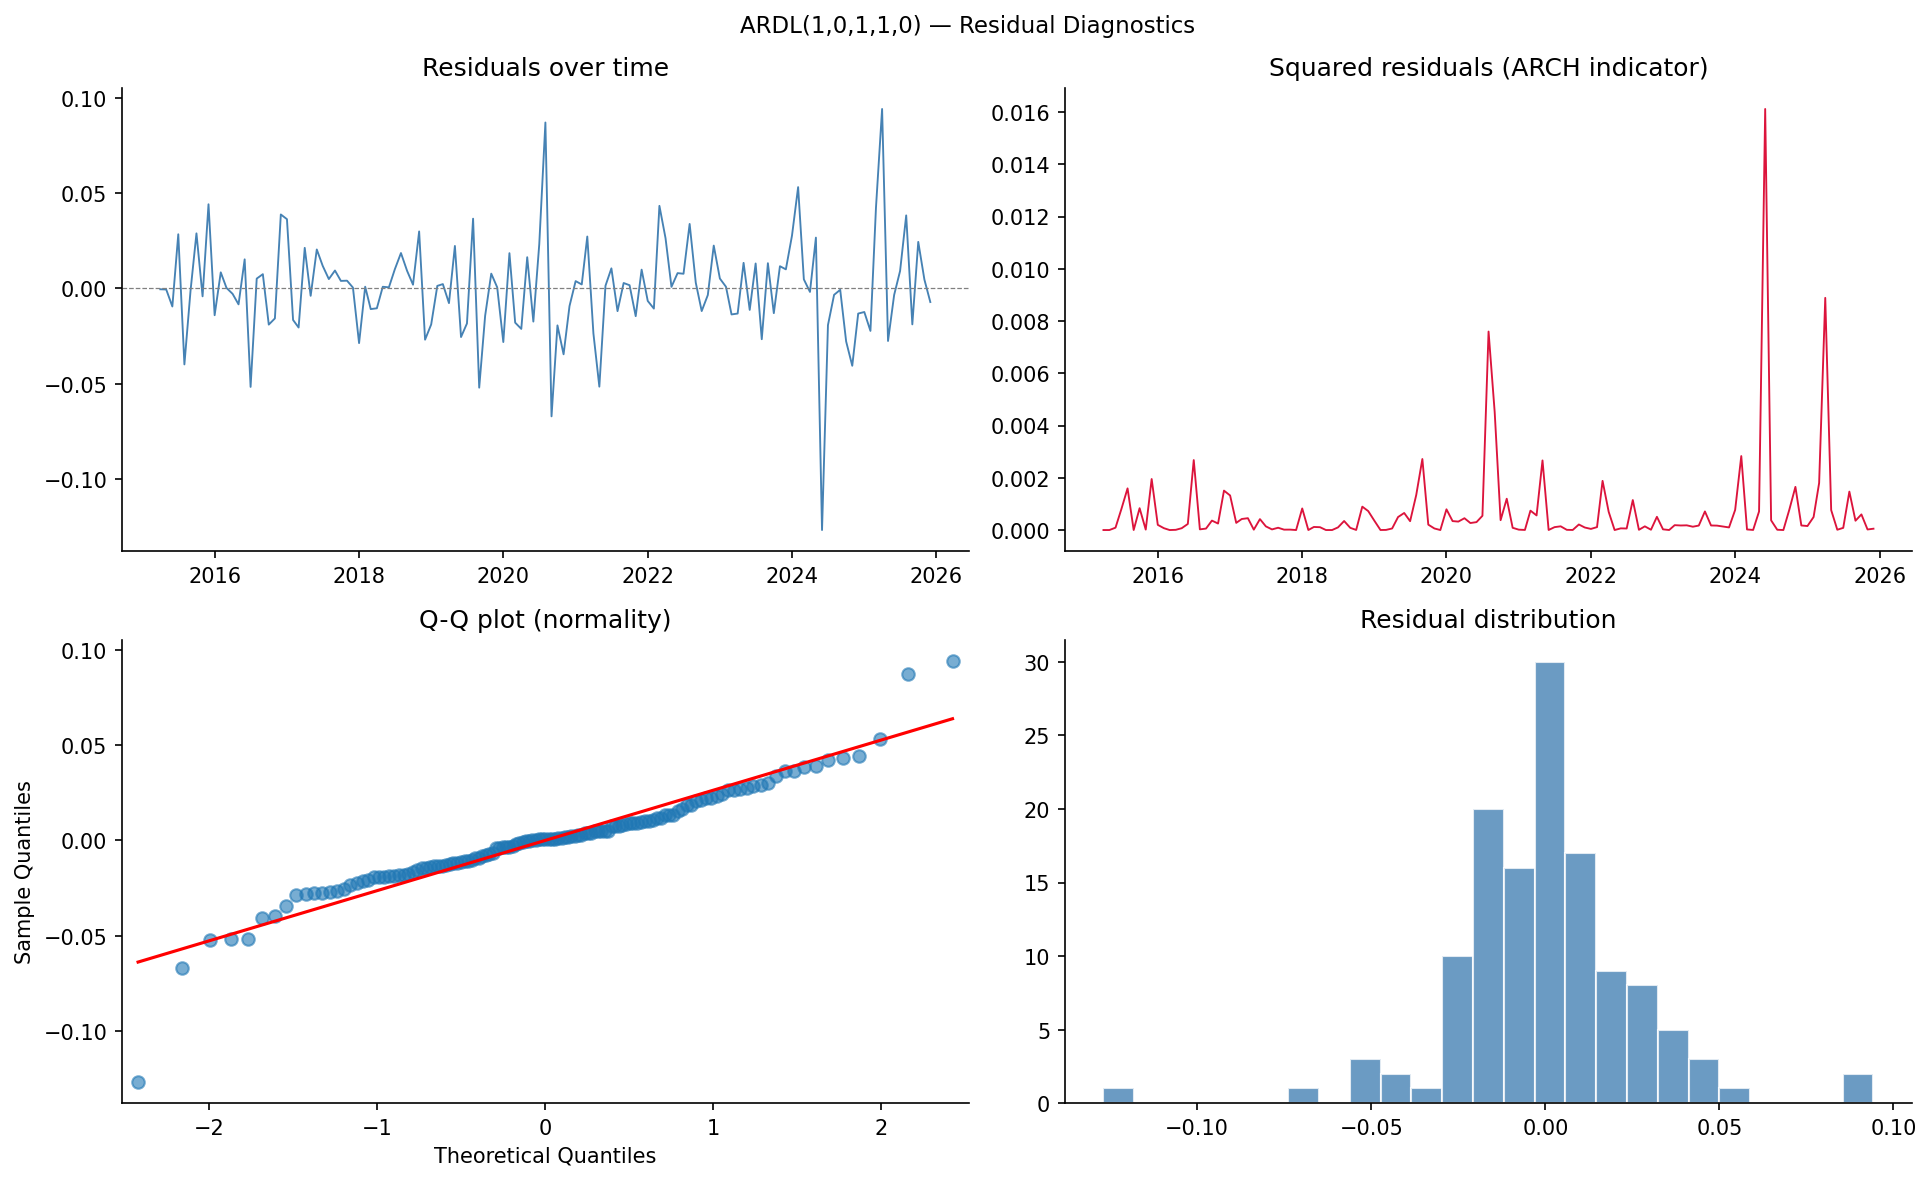
\includegraphics[width=0.92\textwidth]{vietnam_gold_data/manuscript/Figure3_ARDL_diagnostics.png}
\caption{ARDL(1,0,1,1,0) residual diagnostic plots.
\textit{Top left}: residuals over time --- no visible systematic pattern.
\textit{Top right}: squared residuals (ARCH indicator) --- isolated spikes
at 2020 and 2024 are absorbed by $D_{\text{covid}}$ and $D_{\text{sbv24}}$.
\textit{Bottom left}: Q-Q plot --- mild fat tails consistent with the
Jarque-Bera result.
\textit{Bottom right}: residual distribution --- approximately symmetric
around zero.}
\label{fig:ardldiag}
\end{figure}

\subsection{ARIMA order selection and in-sample fit}

Table~\ref{tab:arima} reports the AIC-based order selection across all
nine ARIMA$(p,1,q)$ specifications.

\begin{table}[H]
\caption{ARIMA order selection, $\Delta\ln SJC_t$, training sample 2015:01--2024:12}
\label{tab:arima}
\centering
\small
\begin{tabular}{lccccc}
\toprule
Model & $p$ & $q$ & AIC & BIC & Log-likelihood \\
\midrule
\textbf{ARIMA(0,1,0)} & \textbf{0} & \textbf{0} & \textbf{$-$476.45} & \textbf{$-$473.67} & \textbf{239.22} \\
ARIMA(0,1,1) & 0 & 1 & $-$475.12 & $-$469.56 & 239.56 \\
ARIMA(1,1,0) & 1 & 0 & $-$474.89 & $-$469.33 & 239.45 \\
ARIMA(1,1,1) & 1 & 1 & $-$474.03 & $-$465.69 & 240.01 \\
ARIMA(0,1,2) & 0 & 2 & $-$473.21 & $-$464.87 & 239.61 \\
ARIMA(2,1,0) & 2 & 0 & $-$472.98 & $-$464.64 & 239.49 \\
ARIMA(2,1,1) & 2 & 1 & $-$472.07 & $-$460.95 & 240.03 \\
ARIMA(1,1,2) & 1 & 2 & $-$472.07 & $-$460.95 & 240.03 \\
ARIMA(2,1,2) & 2 & 2 & $-$471.10 & $-$457.21 & 240.55 \\
\bottomrule
\end{tabular}
\begin{minipage}{\linewidth}
\vspace{4pt}
\footnotesize
\textit{Notes}: $d = 1$ fixed from unit root results.
Bold row is selected specification.
Training sample: January 2015 -- December 2024 ($N = 120$).
\end{minipage}
\end{table}

ARIMA(0,1,0) --- a random walk with drift --- achieves the lowest AIC
($-476.45$), confirming no exploitable AR or MA structure in
$\Delta\ln SJC_t$ beyond the most recent observation. The AIC gap
between ARIMA(0,1,0) and the next-best ARIMA(0,1,1) is approximately
1.3 points, sufficient to prefer the more parsimonious specification.
The robustness check confirms ARIMA(1,1,1) AIC = $-474.03$ is inferior.

This result is consistent with the weak-form Efficient Market Hypothesis:
past SJC gold price changes contain no incremental information for
predicting future changes \citep{fama1970}. It implies that any forecasting
improvement from ARIMAX models arises entirely from the macro exogenous
variables, not from autocorrelation in returns.
Figure~\ref{fig:acfpacf} provides the visual confirmation.

\begin{figure}[H]
\centering
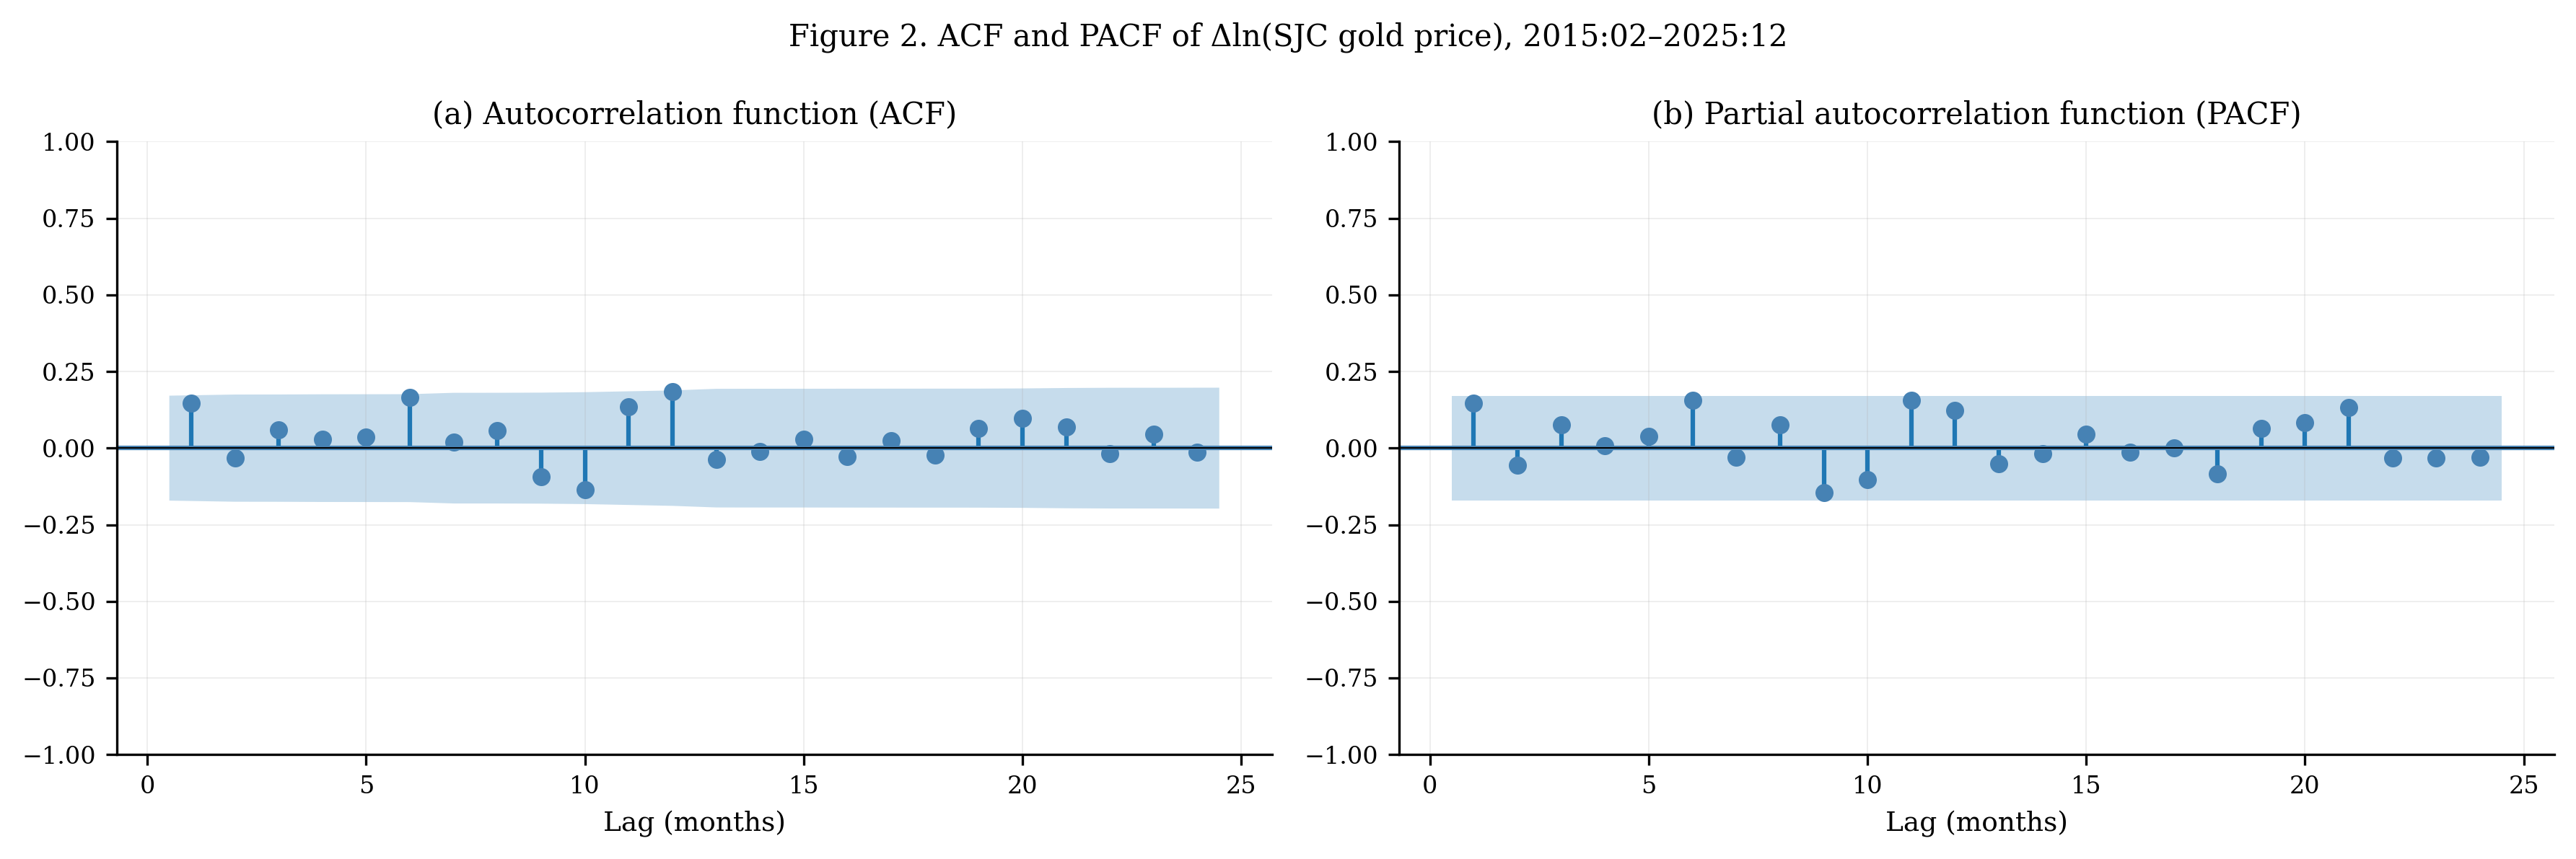
\includegraphics[width=\textwidth]{vietnam_gold_data/manuscript/Figure2_ACF_PACF.png}
\caption{ACF and PACF of $\Delta\ln SJC_t$, 2015:02--2025:12.
Nearly all spikes lie within the 95\% confidence bands (shaded region).
The absence of significant autocorrelation at any lag confirms no
exploitable AR or MA structure, directly supporting the ARIMA(0,1,0)
random walk selection.}
\label{fig:acfpacf}
\end{figure}

\subsection{Forecasting results}

Table~\ref{tab:forecast} presents the out-of-sample forecast accuracy over
the January to December 2025 hold-out period ($h = 12$ months);
Figure~\ref{fig:forecasts} plots the forecast paths against the actual series.

\begin{table}[H]
\caption{Out-of-sample forecast accuracy, January--December 2025 ($h=12$)}
\label{tab:forecast}
\centering
\small
\begin{tabular}{lcccccc}
\toprule
& \multicolumn{3}{c}{Log-level errors} & \multicolumn{3}{c}{VND errors} \\
\cmidrule(lr){2-4}\cmidrule(lr){5-7}
Model & RMSE & MAE & MAPE (\%) & RMSE (M) & MAE (M) & MAPE (\%) \\
\midrule
ARIMA(0,1,0) & 0.3873 & 0.3406 & 1.82 & 43.47 & 37.35 & 27.62 \\
ARIMAX-EX & 0.3311 & 0.2903 & 1.55 & 38.40 & 32.84 & 24.23 \\
ARIMAX-GW & 0.3307 & 0.2903 & 1.55 & 38.36 & 32.84 & 24.24 \\
ARIMAX-BOTH & \textbf{0.3306} & \textbf{0.2901} & \textbf{1.55} & \textbf{38.36} & \textbf{32.81} & \textbf{24.22} \\
\bottomrule
\end{tabular}
\begin{minipage}{\linewidth}
\vspace{4pt}
\footnotesize
\textit{Notes}: RMSE and MAE in log units (columns 2--4) and million VND
per tael (columns 5--7). MAPE = mean absolute percentage error.
Training: January 2015 -- December 2024; Test: January -- December 2025.
Bold row is the best-performing specification. All ARIMAX models reduce
RMSE by 14.5\% and MAPE by 14.9\% relative to the random walk baseline.
\end{minipage}
\end{table}

\paragraph{Diebold-Mariano test.}
Table~\ref{tab:dm} reports the HLN-corrected Diebold-Mariano statistics
testing whether ARIMAX specifications significantly outperform the
ARIMA(0,1,0) random walk baseline.

\begin{table}[H]
\caption{Diebold-Mariano test of equal forecast accuracy}
\label{tab:dm}
\centering
\small
\begin{tabular}{lccl}
\toprule
Challenger model & DM statistic & $p$-value & Decision \\
\midrule
ARIMAX-EX & 4.043 & 0.002 & Reject $H_0$ at 1\%\sig{***} \\
ARIMAX-GW & 4.002 & 0.002 & Reject $H_0$ at 1\%\sig{***} \\
ARIMAX-BOTH & 4.042 & 0.002 & Reject $H_0$ at 1\%\sig{***} \\
\bottomrule
\end{tabular}
\begin{minipage}{\linewidth}
\vspace{4pt}
\footnotesize
\textit{Notes}: HLN small-sample correction applied \citep{harvey1997}.
Positive DM statistic indicates the challenger model has smaller
squared forecast errors than the ARIMA baseline.
*** $p<0.01$; ** $p<0.05$; * $p<0.10$.
All three ARIMAX specifications reject equal forecast accuracy at the 1\%
level. The near-identical DM statistics across ARIMAX-EX, ARIMAX-GW,
and ARIMAX-BOTH suggest that the forecast gains are driven mainly by the
shared information in world gold prices and the exchange rate jointly.
\end{minipage}
\end{table}

\begin{figure}[htbp]
\centering
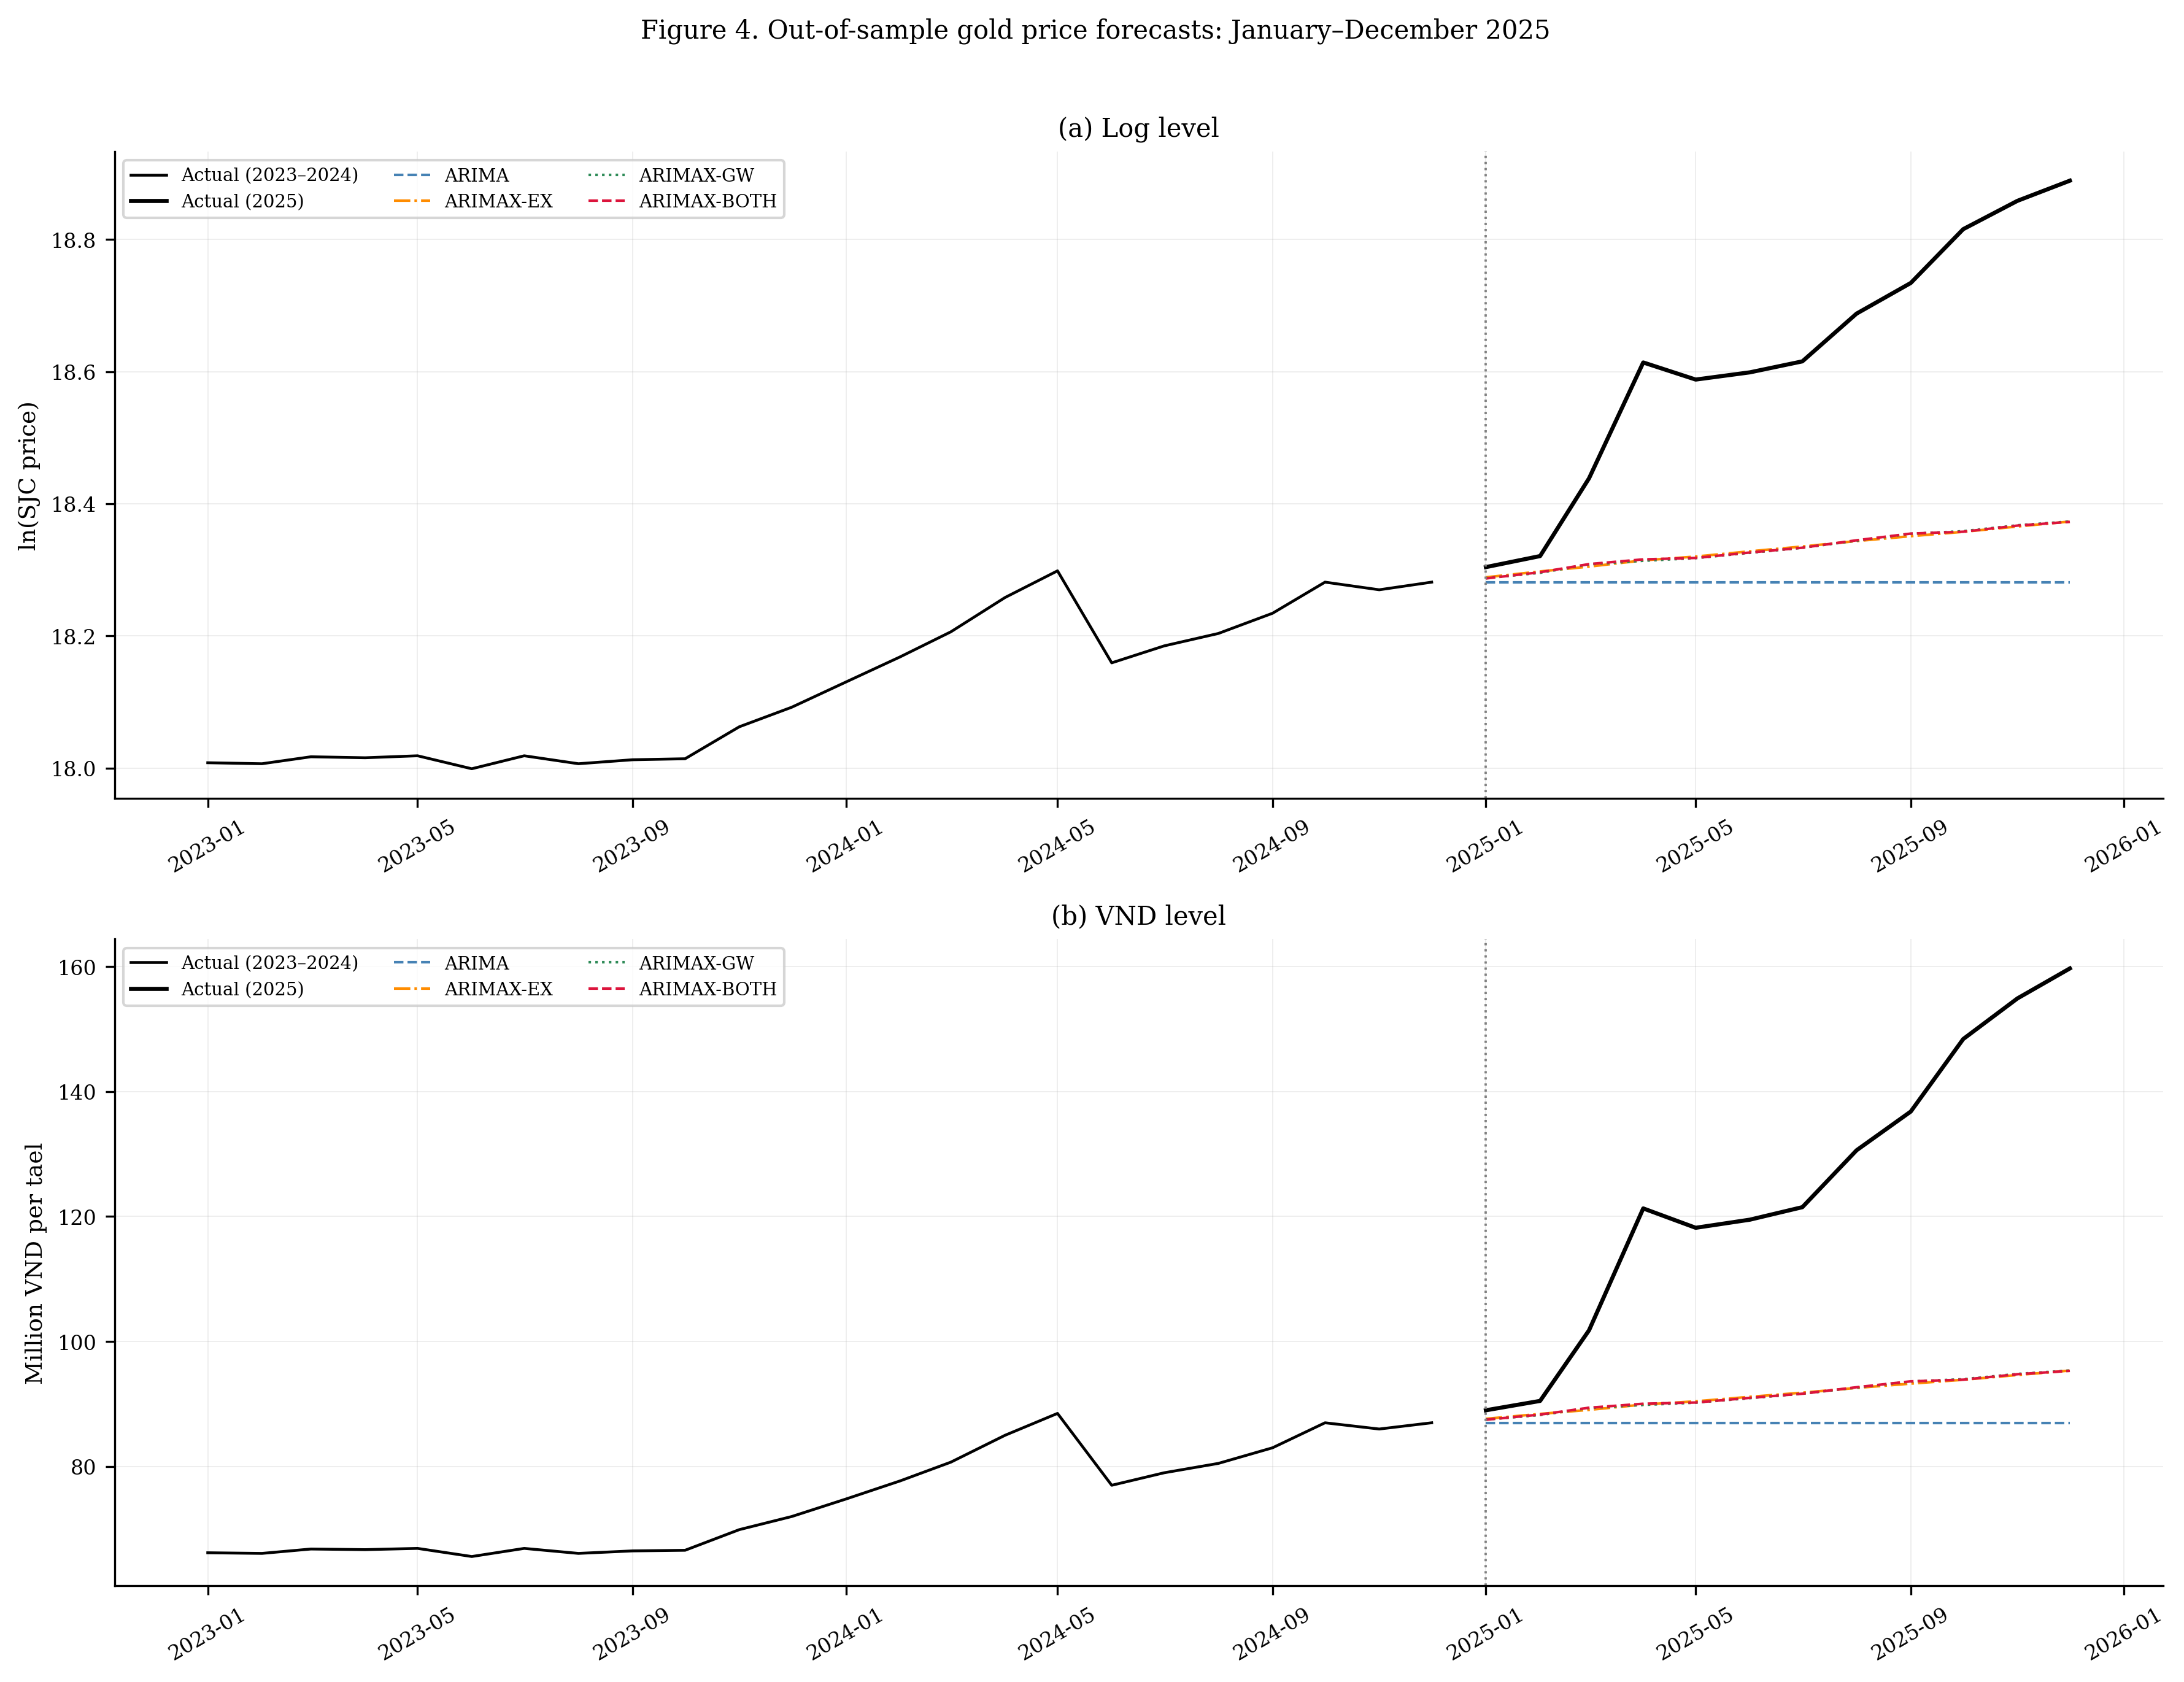
\includegraphics[width=0.95\textwidth]{vietnam_gold_data/manuscript/Figure4_forecasts_2025.png}
\caption{Out-of-sample gold price forecasts, January -- December 2025.
Panel (a): log SJC price level. Panel (b): million VND per tael.
The vertical dotted line marks the forecast origin (end of training sample).
All four models substantially underpredict the actual 2025 price surge,
reflecting the unprecedented post-reform appreciation (SJC exceeded
160 million VND/tael by end-2025) not captured by the linear
time-series structure estimated on 2015--2024 data.}
\label{fig:forecasts}
\end{figure}

%───────────────────────────────────────────────────────────────────────────────
\section{Discussion}
\label{sec:discussion}
%───────────────────────────────────────────────────────────────────────────────

\subsection{Long-run price determination}

The statistically insignificant but theoretically consistent long-run
coefficients suggest that the fundamental drivers of SJC gold prices ---
exchange rate, world gold price, inflation, and interest rates --- operate
through the hypothesised channels but cannot be precisely estimated from
the available monthly panel.
This finding is consistent with the literature on small-sample ARDL studies
\citep{pesaran2001, rana2023} and does not imply the absence of long-run
relationships; rather, it reflects the inherent power limitations when
$T \approx 130$.

The negative long-run exchange rate coefficient ($-0.995$, $n.s.$) requires
careful interpretation. While the sign contradicts the simple PPP prediction,
the wide confidence interval ([$-4.25$, $+2.26$]) spans both positive and
negative values, indicating that the point estimate is not distinguishable
from the theoretically expected positive value. The SBV's active management
of the USD/VND rate may compress the long-run co-movement between exchange
rate and gold price, explaining why the long-run pass-through is weaker
than the short-run estimate.

\subsection{Short-run dynamics and policy implications}

The short-run results have direct implications for market participants.
First, the full contemporaneous pass-through from exchange rate to gold
price ($\beta = 1.039$) implies that hedging domestic gold price risk
through currency derivatives provides near-complete coverage in the same
month. Portfolio managers holding SJC gold should therefore monitor
USD/VND rate movements as a leading indicator of within-month price
changes.

Second, the dominant role of world gold price changes ($\beta = 0.504$
contemporaneous, $\beta = 0.345$ lagged) suggests that Vietnamese gold
markets are significantly integrated with global markets despite the
historical SJC premium. The two-month transmission window (current plus
lagged) is consistent with a market that is informally segmented but
not structurally isolated from global pricing signals.

Third, the error correction speed of 14.1\% per month (half-life 4.6 months)
indicates that while short-run deviations from long-run equilibrium are
gradually corrected, they persist for meaningful durations. This
persistence creates window-dressing opportunities for short-term gold
traders and complicates the SBV's ability to manage domestic gold prices
purely through monetary policy.

\subsection{EMH implications from ARIMA results}

The ARIMA(0,1,0) selection implies that the Vietnamese gold market satisfies
the weak form of the Efficient Market Hypothesis \citep{fama1970}: all
information in the history of past SJC prices is already incorporated
in the current price. This is a stronger statement than the cointegration
results, which concern long-run equilibria. The combined findings suggest
a market that is informationally efficient in the short run but may exhibit
systematic mean-reversion at longer horizons (captured by the ECT).

The Diebold-Mariano test results sharply reject the null of equal forecast
accuracy for all three ARIMAX specifications (DM $\approx 4.04$,
$p \approx 0.002$). This finding implies that the Vietnamese gold market
is not semi-strong form efficient with respect to publicly available
exchange rate and world gold price information: incorporating these
variables into the forecasting model yields statistically and economically
significant improvements over a random walk. The MAPE reduction of 14.9\%
(from 1.82\% to 1.55\%) translates into approximately 4.5 million VND
per tael in mean absolute forecast error, which is economically meaningful
for portfolio managers and traders operating in the Vietnamese gold market.

The combination of weak-form efficiency (random walk univariate model) and
semi-strong-form inefficiency (ARIMAX outperforms) is internally consistent:
past SJC gold returns contain no information (weak-form), but contemporaneous
macro variables --- particularly world gold price changes and USD/VND
depreciation --- are not instantaneously and fully incorporated into SJC
prices. This creates a one-period informational lag that ARIMAX exploits.
The finding is consistent with \citet{wang2021}, who document that gold
markets in managed-rate economies exhibit partial, not complete, integration
with global price signals.

\subsection{Structural stability and the SBV reform}

Both Chow structural break tests pass comfortably ($p = 0.467$ for COVID;
$p = 0.600$ for SBV reform), indicating that the ARDL coefficients are
stable across the two regime shifts. This is a substantive result: it
implies that the fundamental short-run relationships between SJC gold
and macroeconomic variables were not altered by the 2024 auction reform,
despite its dramatic effect on the SJC premium level. The reform changed
the \textit{level} of the domestic price (captured by $D_{\text{sbv24}}$)
without altering the \textit{dynamic} relationships.

%───────────────────────────────────────────────────────────────────────────────
\section{Conclusion}
\label{sec:conclusion}
%───────────────────────────────────────────────────────────────────────────────

This paper examines the macroeconomic determinants of domestic SJC gold
prices in Vietnam over the period January 2015 to December 2025, combining
ARDL bounds testing with ARIMA/ARIMAX out-of-sample forecasting. Our principal
findings are as follows.

First, using ARDL bounds testing, we confirm cointegration at the 1\%
significance level (F = 5.229, $p = 0.0002$), supported by a significant
error correction term (ECT = $-0.141$, $p = 0.016$), with 14.1\% of
price disequilibria corrected within one month.
All four long-run coefficients carry the theoretically predicted signs,
although sample-size limitations preclude individual significance.

Second, in the short run, world gold price changes are the dominant driver
of SJC price movements, with a contemporaneous elasticity of 0.504 ($p < 0.001$)
and a lagged effect of 0.345 ($p < 0.001$). USD/VND exchange rate depreciation
exerts a full short-run pass-through ($\beta = 1.039$, $p = 0.027$),
consistent with purchasing power parity at the monthly frequency.

Third, ARIMA order selection identifies a random walk as the optimal
univariate model, supporting weak-form market efficiency for the Vietnamese
gold market. However, ARIMAX models incorporating world gold price changes
and the USD/VND exchange rate significantly outperform the random walk
baseline (DM $\approx 4.04$, $p < 0.01$), indicating that the market is
not semi-strong form efficient with respect to publicly available macro
information.

Fourth, structural stability is confirmed across both the COVID-19 shock
and the SBV gold market reform, suggesting that the reform altered price
\textit{levels} without disrupting the underlying dynamic transmission
mechanisms.

\paragraph{Policy implications.}
For the SBV, the results suggest that exchange rate management
has an immediate and near-complete effect on domestic gold prices,
implying that episodes of rapid VND depreciation will translate directly
into gold price surges. The persistence of the ECT (half-life 4.6 months)
indicates a moderate degree of market efficiency that limits the effectiveness
of short-term interventions.
For investors, the findings confirm gold's role as an inflation hedge and
currency risk hedger in Vietnam, with world gold price movements providing
the primary return signal at monthly frequencies.

\paragraph{Limitations and future research.}
This study faces three limitations.
First, the constructed CPI series (annual data compounded to monthly) may
understate true monthly inflation volatility.
Second, the 2025 SJC price data for some months rely on estimates rather
than official records; future work should verify these values.
Third, the small sample ($T = 132$) limits the power of long-run inference.
Future research could extend the sample horizon, incorporate GARCH-class
volatility models to address the documented ARCH effects, or explore
nonlinear cointegration methods to examine whether the long-run equilibrium
relationship is regime-dependent.

%───────────────────────────────────────────────────────────────────────────────
\newpage
\bibliographystyle{apalike}
\begin{thebibliography}{99}

\bibitem[Bahmani-Oskooee and Harvey(2016)]{bahmani2016}
Bahmani-Oskooee, M., \& Harvey, H. (2016).
Exchange rate sensitivity of U.S. bilateral trade flows.
\textit{Economic Modelling}, 53, 329--337.

\bibitem[Baur and McDermott(2010)]{baur2010}
Baur, D.~G., \& McDermott, T.~K. (2010).
Is gold a safe haven? International evidence.
\textit{Journal of Banking \& Finance}, 34(8), 1886--1898.

\bibitem[Derbali(2021)]{derbali2021}
Derbali, A. (2021).
Drivers of gold returns: Evidence from COVID-19 pandemic.
\textit{Journal of Public Affairs}, 21(3), e2368.

\bibitem[Diebold and Mariano(1995)]{diebold1995}
Diebold, F.~X., \& Mariano, R.~S. (1995).
Comparing predictive accuracy.
\textit{Journal of Business \& Economic Statistics}, 13(3), 253--263.

\bibitem[Dickey and Fuller(1981)]{dickey1981}
Dickey, D.~A., \& Fuller, W.~A. (1981).
Likelihood ratio statistics for autoregressive time series with a unit root.
\textit{Econometrica}, 49(4), 1057--1072.

\bibitem[Do et al.(2023)]{do2023}
Do, T.~T., Tran, T.~H., Nguyen, T.~T., Le, A.~T., \& Ninh, L.~K. (2023).
Is gold an inflation hedge in Vietnam? A non-linear approach.
\textit{Cogent Economics \& Finance}, 11(2), 2244857.
https://doi.org/10.1080/23322039.2023.2244857

\bibitem[Fama(1970)]{fama1970}
Fama, E.~F. (1970).
Efficient capital markets: A review of theory and empirical work.
\textit{Journal of Finance}, 25(2), 383--417.

\bibitem[Hammoudeh and Yuan(2008)]{hammoudeh2010}
Hammoudeh, S., \& Yuan, Y. (2008).
Metal volatility in presence of oil and interest rate shocks.
\textit{Energy Economics}, 30(2), 606--620.

\bibitem[Harvey et al.(1997)]{harvey1997}
Harvey, D., Leybourne, S., \& Newbold, P. (1997).
Testing the equality of prediction mean squared errors.
\textit{International Journal of Forecasting}, 13(2), 281--291.

\bibitem[Kremers et al.(1992)]{kremers1992}
Kremers, J.~J., Ericsson, N.~R., \& Dolado, J.~J. (1992).
The power of cointegration tests.
\textit{Oxford Bulletin of Economics and Statistics}, 54(3), 325--348.

\bibitem[Kwiatkowski et al.(1992)]{kwiatkowski1992}
Kwiatkowski, D., Phillips, P.~C.~B., Schmidt, P., \& Shin, Y. (1992).
Testing the null hypothesis of stationarity against the alternative of a unit root.
\textit{Journal of Econometrics}, 54(1--3), 159--178.

\bibitem[Nguyen and Tran(2020)]{nguyen2020}
Nguyen, V.~H., \& Tran, T.~Q. (2020).
Exchange rate uncertainty and gold prices in Vietnam: A GARCH approach.
\textit{Journal of Economics and Development}, 22(1), 45--58.

\bibitem[Pesaran et al.(2001)]{pesaran2001}
Pesaran, M.~H., Shin, Y., \& Smith, R.~J. (2001).
Bounds testing approaches to the analysis of level relationships.
\textit{Journal of Applied Econometrics}, 16(3), 289--326.

\bibitem[Phillips and Perron(1988)]{phillips1988}
Phillips, P.~C.~B., \& Perron, P. (1988).
Testing for a unit root in time series regression.
\textit{Biometrika}, 75(2), 335--346.

\bibitem[Pierdzioch et al.(2016)]{pierdzioch2016}
Pierdzioch, C., Risse, M., \& Rohloff, S. (2016).
Are gold price forecasts more accurate when exchange rates are included?
\textit{Empirical Economics}, 50(2), 477--500.

\bibitem[Rana and O'Connor(2023)]{rana2023}
Rana, F., \& O'Connor, F.~A. (2023).
Domestic macroeconomic determinants of precious metals prices in developed
and emerging markets.
\textit{International Review of Financial Analysis}, 89, 102813.
https://doi.org/10.1016/j.irfa.2023.102813

\bibitem[Sahu et al.(2022)]{sahu2022}
Sahu, T.~N., Mondal, P., \& Bandopadhyay, K. (2022).
Nexus between gold prices, exchange rates and stock markets.
\textit{Journal of Financial Economic Policy}, 14(3), 415--432.

\bibitem[Salisu et al.(2021)]{salisu2021}
Salisu, A.~A., Raheem, I.~D., \& Ndako, U.~B. (2021).
A sectoral analysis of asymmetric nexus between oil price and stock returns.
\textit{International Review of Economics \& Finance}, 73, 252--265.

\bibitem[Tran et al.(2021)]{tran2021}
Tran, M.~T., Nguyen, T.~H., \& Le, P.~T. (2021).
Gold as an inflation hedge in Vietnam: Time-horizon analysis.
\textit{Finance Research Letters}, 40, 101683.

\bibitem[Tully and Lucey(2007)]{tully2007}
Tully, E., \& Lucey, B.~M. (2007).
A power GARCH examination of the gold market.
\textit{Research in International Business and Finance}, 21(2), 316--325.

\bibitem[Wang et al.(2021)]{wang2021}
Wang, Y., Wei, Y., Wu, C., \& Yin, L. (2021).
Is gold a safe haven for the dynamic risk of foreign exchange?
\textit{Future Business Journal}, 7(1), 56.
https://doi.org/10.1186/s43093-021-00101-9

\bibitem[World Gold Council(2023)]{worldgoldcouncil2023}
World Gold Council. (2023).
\textit{Gold Demand Trends Full Year 2022}.
London: World Gold Council.

\bibitem[Zivot and Andrews(1992)]{zivot1992}
Zivot, E., \& Andrews, D.~W.~K. (1992).
Further evidence on the great crash, the oil price shock, and the unit root hypothesis.
\textit{Journal of Business \& Economic Statistics}, 10(3), 251--270.

\end{thebibliography}

%───────────────────────────────────────────────────────────────────────────────
\newpage
\appendix
%───────────────────────────────────────────────────────────────────────────────

\section{Full ECM Coefficient Table}
\label{app:ecm}

Table~\ref{tab:ecm_full} reports all estimated coefficients from the
ARDL(1,0,1,1,0) model. Short-run terms not reaching conventional significance
thresholds are included for completeness.

\begin{table}[H]
\caption{Full ECM coefficient estimates, ARDL(1,0,1,1,0)}
\label{tab:ecm_full}
\centering
\small
\begin{tabular}{lcccc}
\toprule
Variable & Coefficient & Std.\ Error (HAC) & $t$-stat & $p$-value \\
\midrule
Constant & $+1.9834$ & $1.6981$ & $+1.168$ & $0.243$ \\
$D_{\text{covid}}$ & $-0.0088$ & $0.0136$ & $-0.645$ & $0.519$ \\
$D_{\text{sbv24}}$ & $-0.0019$ & $0.0180$ & $-0.107$ & $0.914$ \\
$D_{\text{tet}}$ & $-0.0016$ & $0.0059$ & $-0.265$ & $0.791$ \\
ECT ($\ln SJC_{t-1}$) & $-0.1410^{**}$ & $0.0586$ & $-2.409$ & $0.016$ \\
$\ln EXRATE_{t-1}$ & $-0.1403$ & $0.1994$ & $-0.704$ & $0.482$ \\
$\ln GOLD_{W,t-1}$ & $+0.1677^{**}$ & $0.0711$ & $+2.358$ & $0.018$ \\
$\ln CPI_{t-1}$ & $+0.1539$ & $0.1201$ & $+1.282$ & $0.200$ \\
$IR_{t-1}$ & $-0.0044$ & $0.0057$ & $-0.766$ & $0.444$ \\
$\Delta\ln SJC_{t-1}$ & $-0.1340^{**}$ & $0.0634$ & $-2.115$ & $0.035$ \\
$\Delta\ln EXRATE_t$ & $+1.0391^{**}$ & $0.4004$ & $+2.595$ & $0.010$ \\
$\Delta\ln GOLD_{W,t}$ & $+0.5044^{***}$ & $0.0959$ & $+5.260$ & $0.000$ \\
$\Delta\ln GOLD_{W,t-1}$ & $+0.3445^{***}$ & $0.1040$ & $+3.311$ & $0.001$ \\
$\Delta\ln CPI_t$ & $+20.059^{**}$ & $8.860$ & $+2.264$ & $0.024$ \\
$\Delta\ln CPI_{t-1}$ & $-23.361^{***}$ & $7.989$ & $-2.924$ & $0.004$ \\
$\Delta IR_t$ & $+0.0256^{**}$ & $0.0106$ & $+2.409$ & $0.016$ \\
\midrule
$N$ & 129 & $R^2$ & 0.4719 & \\
$\text{Adj.}\ R^2$ & 0.4018 & AIC & $-539.809$ & \\
\bottomrule
\end{tabular}
\begin{minipage}{\linewidth}
\vspace{4pt}
\footnotesize
\textit{Notes}: *** $p<0.01$; ** $p<0.05$; * $p<0.10$. HAC (Newey-West) robust
standard errors throughout. Long-run levels coefficients ($\ln EXRATE_{t-1}$
through $IR_{t-1}$) combine with ECT to recover the cointegrating vector.
Significance of $\ln GOLD_{W,t-1}$ (p=0.018) in the levels equation reflects
long-run world gold price transmission.
\end{minipage}
\end{table}

\section{SBV Refinancing Rate Schedule}
\label{app:ir}

Table~\ref{tab:ir} documents the SBV refinancing rate schedule used
in the empirical analysis.

\begin{table}[H]
\caption{SBV refinancing rate schedule, 2015--2025}
\label{tab:ir}
\centering
\small
\begin{tabular}{llll}
\toprule
Effective date & Rate (\% p.a.) & Decision number & Direction \\
\midrule
January 2015 & 6.50 & Decision 2173/QĐ-NHNN (Oct 2014) & Baseline \\
July 2017 & 6.25 & Decision 1172/QĐ-NHNN, 30 Jun 2017 & Cut \\
October 2017 & 6.00 & SBV announcement, Sep 2017 & Cut \\
March 2020 & 5.00 & Decision 418/QĐ-NHNN, 16 Mar 2020 & Cut (COVID) \\
May 2020 & 4.50 & Decision 919/QĐ-NHNN, 12 May 2020 & Cut \\
October 2020 & 4.00 & Decision 1728/QĐ-NHNN, 30 Sep 2020 & Cut \\
September 2022 & 5.00 & Decision 1606/QĐ-NHNN, 22 Sep 2022 & Hike \\
October 2022 & 6.00 & Decision 1809/QĐ-NHNN, 24 Oct 2022 & Hike \\
April 2023 & 5.50 & Decision 574/QĐ-NHNN, 31 Mar 2023 & Cut \\
May 2023 & 5.00 & Decision 950/QĐ-NHNN, 23 May 2023 & Cut \\
July 2023 & 4.50 & Decision 1123/QĐ-NHNN, 16 Jun 2023 & Cut \\
December 2025 & 4.50 & Unchanged since Jul 2023 & --- \\
\bottomrule
\end{tabular}
\begin{minipage}{\linewidth}
\vspace{4pt}
\footnotesize
\textit{Source}: State Bank of Vietnam official decisions (QĐ-NHNN),
retrieved from sbv.gov.vn.
\end{minipage}
\end{table}

\end{document}